\section{DRIVE Database}

\begin{figure}[h!]
    \centering
    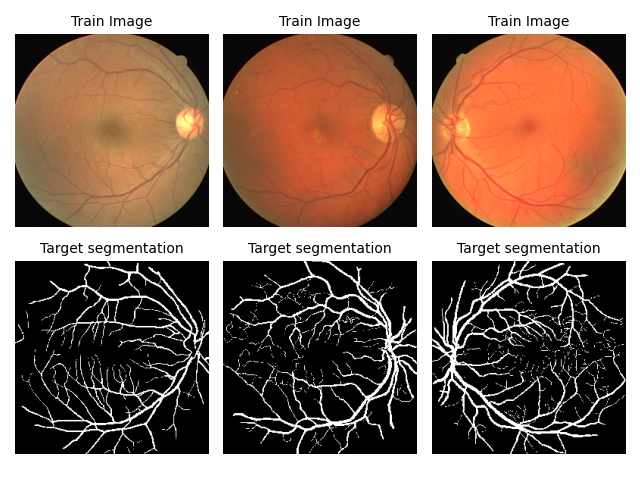
\includegraphics[width=\textwidth]{figures/ex_drive.png}
    \caption{Examples of DRIVE database}
    \label{ex_drive}
\end{figure}
 
\section{Learning curves for DRIVE dataset}

\begin{figure}[H]
    \centering
    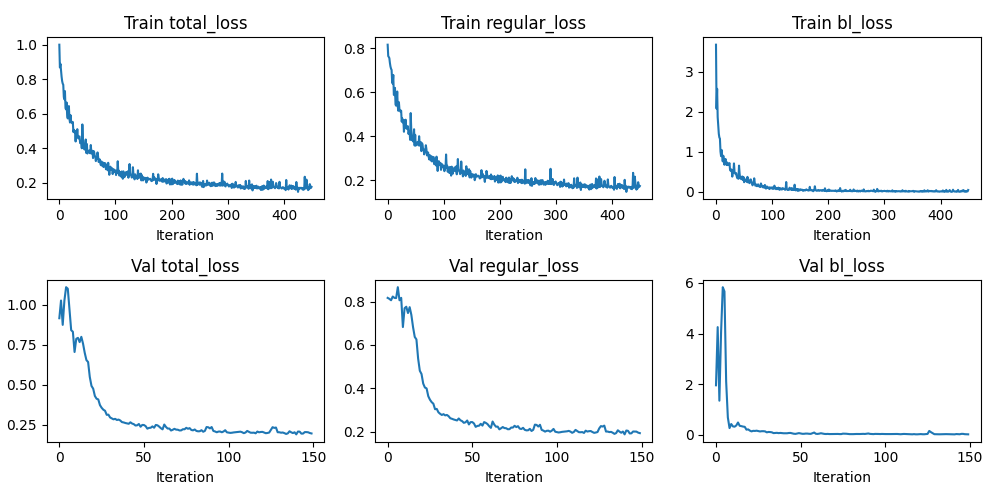
\includegraphics[width=\textwidth]{figures/learning_curves.png}
    \caption{Loss evolution during training of DRIVE dataset with $\lcal_1$. The "regular\_loss" is $\lcal_{GDL}$}
    \label{fig:learn_curves_drive}
\end{figure}

\begin{figure}[H]
    \centering
    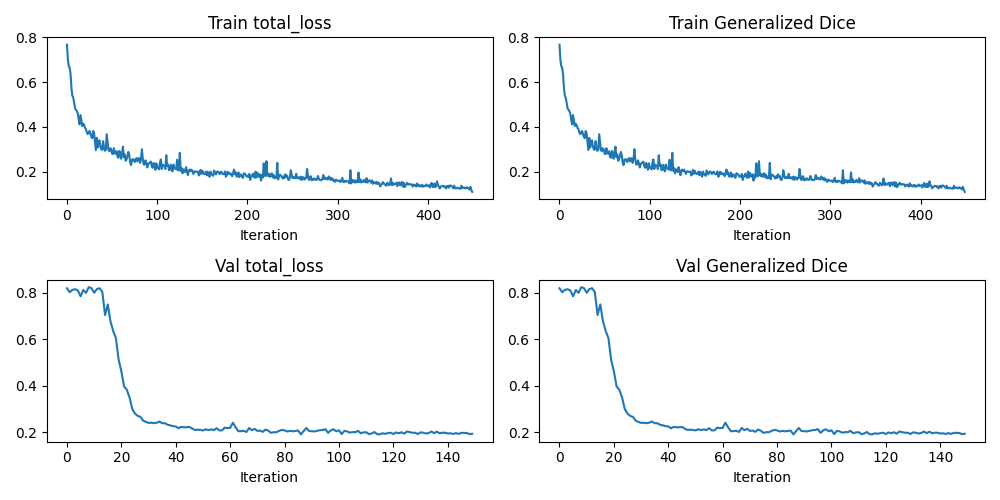
\includegraphics[width=\textwidth]{figures/GDL_learning_curves.png}
    \caption{Loss evolution during training of DRIVE dataset with $\lcal_2$ (without boundary loss)}
    \label{fig:learn_curve_drive_l2}
\end{figure}

\begin{figure}[H]
    \centering
    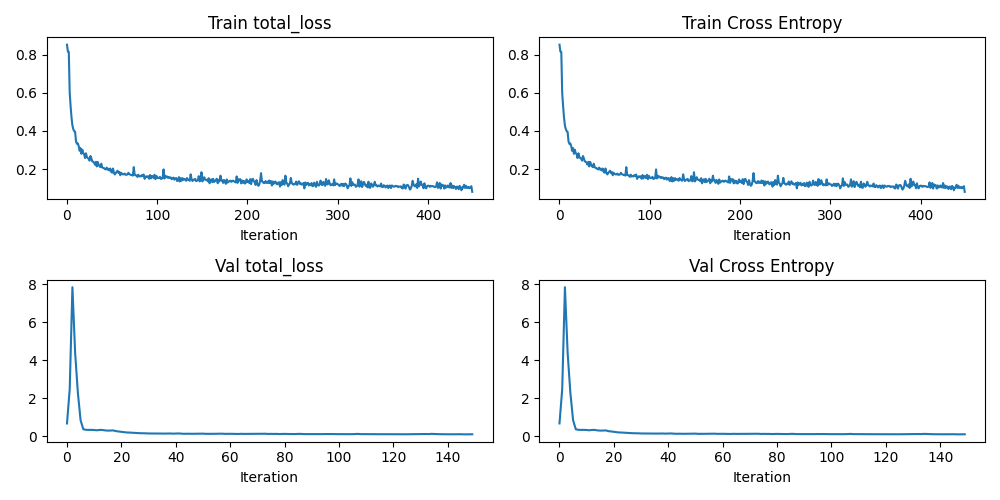
\includegraphics[width=\textwidth]{figures/CE_learning_curves.png}
    \caption{Loss evolution during training of DRIVE dataset with $\lcal_3$}
    \label{fig:learn_drive_l3}
\end{figure}

\begin{figure}[H]
    \centering
    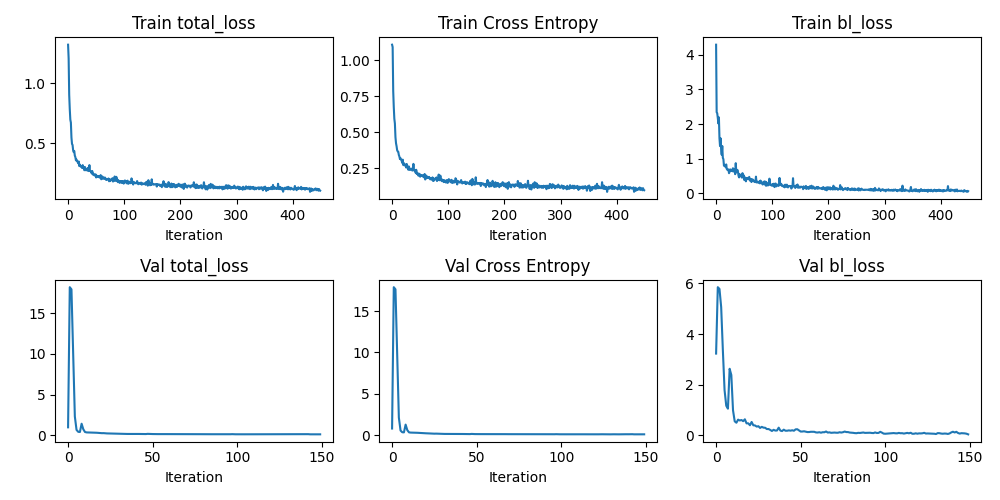
\includegraphics[width=\textwidth]{figures/CEwBL_learning_curves.png}
    \caption{Loss evolution during training of DRIVE dataset with $\lcal_4$}
    \label{fig:learn_drive_l4}
\end{figure}

\section{Dice score on DRIVE dataset}

\begin{figure}[h!]
    \centering
    \begin{subfigure}{0.45\textwidth}
        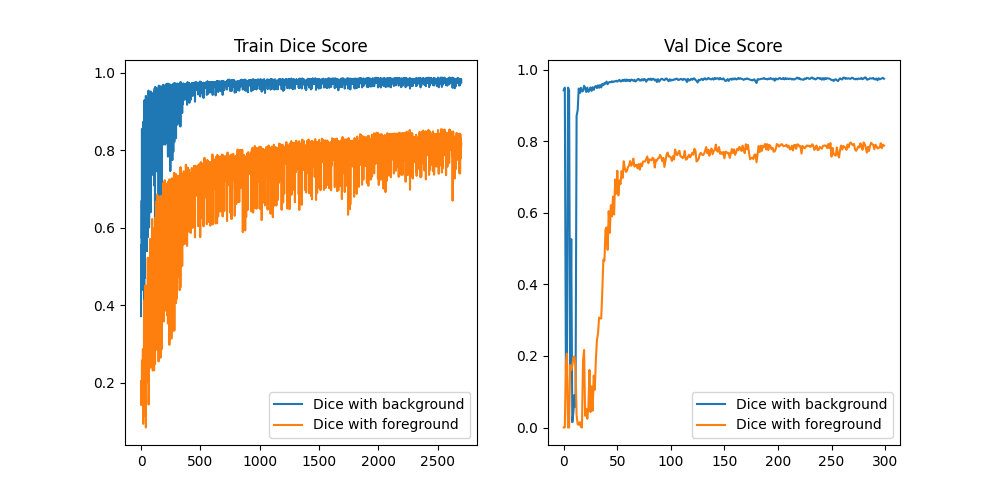
\includegraphics[width=\textwidth]{figures/dice_coeff_training.png}
        \caption{$\lcal_1$}
    \end{subfigure}
    \begin{subfigure}{0.45\textwidth}
        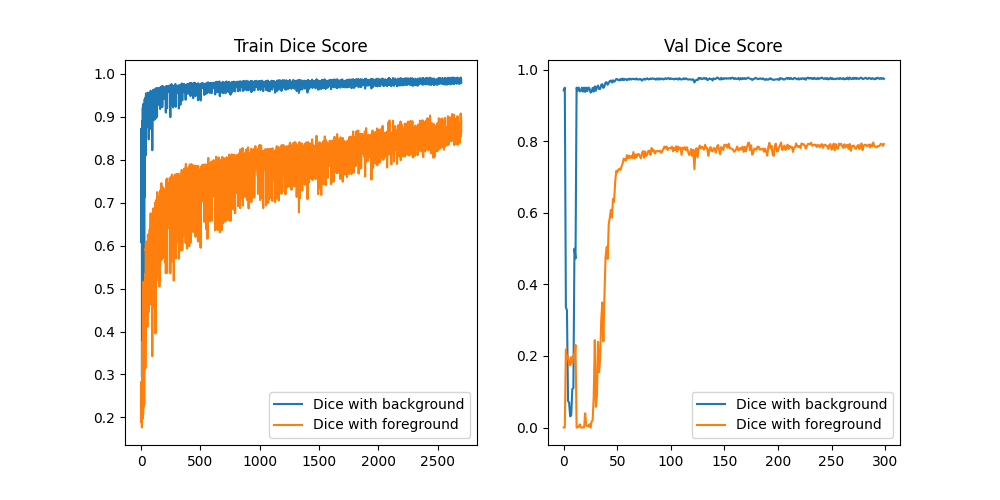
\includegraphics[width=\textwidth]{figures/GDL_dice_coeff_training.png}
        \caption{$\lcal_2$}
    \end{subfigure}
    \begin{subfigure}{0.45\textwidth}
        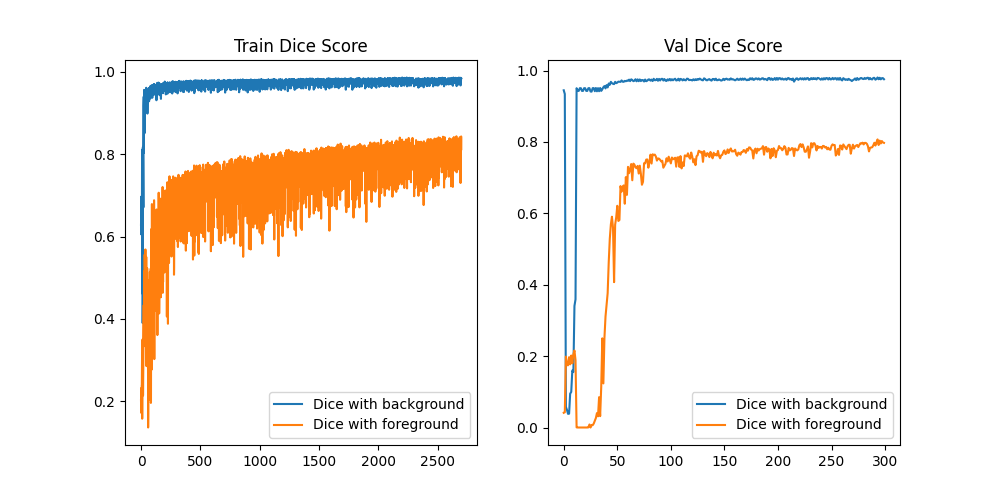
\includegraphics[width=\textwidth]{figures/CE_dice_coeff_training.png}
        \caption{$\lcal_{3}$}
    \end{subfigure}
    \begin{subfigure}{0.45\textwidth}
        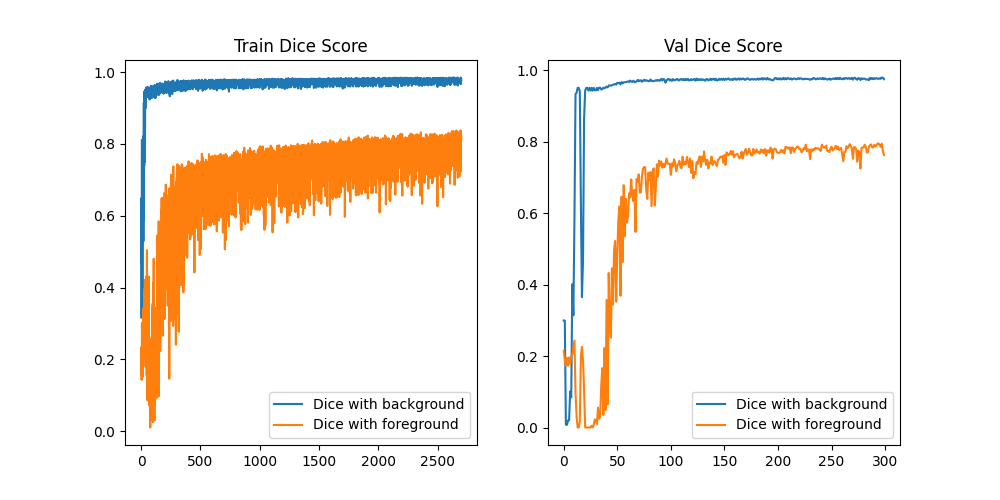
\includegraphics[width=\textwidth]{figures/CEwBL_dice_coeff_training.png}
        \caption{$\lcal_{4}$}
    \end{subfigure}
    \caption{Evolution of the dice score during training on DRIVE dataset} The dice score for the foreground and background are plotted for the training and validation dataset. $\lcal_{1}$, $\lcal_2$ and $\lcal_3$ are the different losses evaluated during the experiments described above. $\lcal_3$ is the "baseline" loss. In our case, it is the cross-entropy loss function.
    \label{fig:dsc_train_drive}
\end{figure}